\documentclass{article}
\usepackage{tikz}
\begin{document}
	\begin{center}
		\Large{\textbf{Hierarchy of Linux distributions}}
	\end{center}
	\begin{figure}[h]
		\centering
		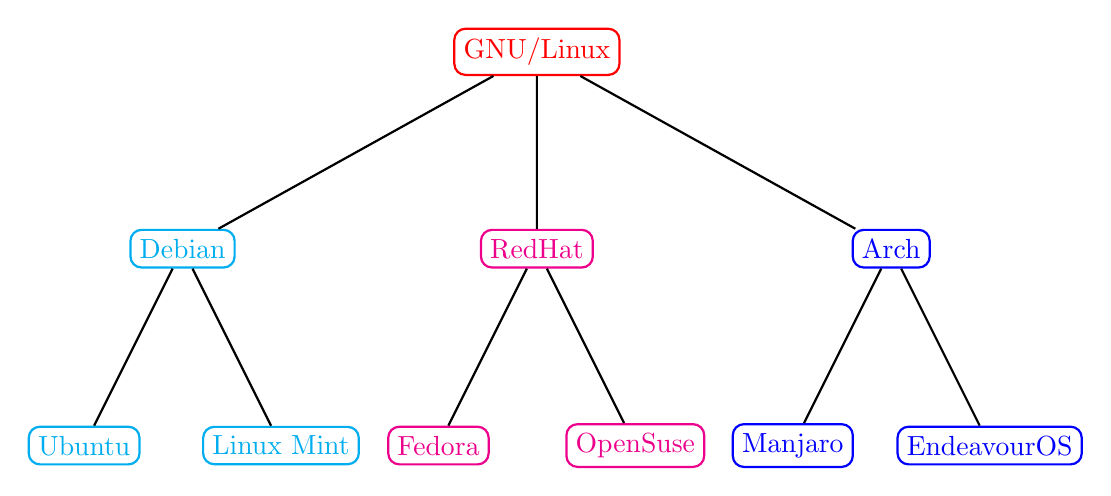
\begin{tikzpicture} [every node/.style = {shape=rectangle, rounded corners, draw,
				align=center}]
			\path [draw,thick,-]
			node (root)[red] {GNU/Linux}
			[sibling distance=45mm, level distance=25mm]
			child {node [cyan] {Debian}
				[sibling distance=25mm, level distance=25mm]
				child { node [cyan] {Ubuntu} }
				child { node [cyan] {Linux Mint} }
			}
			child {node [magenta] {RedHat}
				[sibling distance=25mm, level distance=25mm]
				child { node [magenta] {Fedora} }
				child { node [magenta] {OpenSuse} }
			}
			child {node [blue] {Arch}
				[sibling distance=25mm, level distance=25mm]
				child { node [blue]{Manjaro} }
				child { node [blue]{EndeavourOS} }
			};
			
		\end{tikzpicture}
		\caption{GNU/Linux Operating System Family}
	\end{figure}
	\pagebreak
	\begin{center}
		\Large{\textbf{SUV Cars}}
	\end{center}
	\begin{figure}[h]
		\centering
		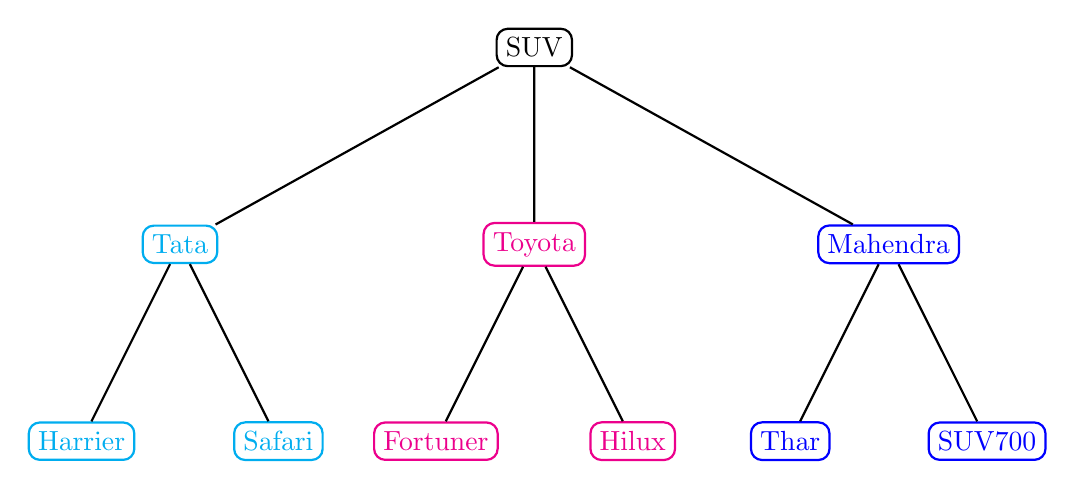
\begin{tikzpicture} [every node/.style = {shape=rectangle, rounded corners, draw,
				align=center}]
			\path [draw,thick,-]
			[grow=-90]
			node (root)[black] {SUV}
			[sibling distance=45mm, level distance=25mm]
			child {node [cyan] {Tata}
				[sibling distance=25mm, level distance=25mm]
				child { node [cyan] {Harrier} }
				child { node [cyan] {Safari} }
				% child { node {Elementary} }
			}
			child {node [magenta] {Toyota}
				[sibling distance=25mm, level distance=25mm]
				child { node [magenta] {Fortuner} }
				child { node [magenta] {Hilux} }
			}
			child {node [blue] {Mahendra}
				[sibling distance=25mm, level distance=25mm]
				child { node [blue]{Thar} }
				child { node [blue]{SUV700} }
			};
			
		\end{tikzpicture}
		\caption{Car Brands Hierarchy}
	\end{figure}
\end{document}